%!TEX root = ../../paper.tex

\begin{figure}[b]
	\centering
	%!TEX root = ../../paper.tex

% Ferdosi Set 2
\begin{subfigure}{0.23\textwidth}
	\centering
	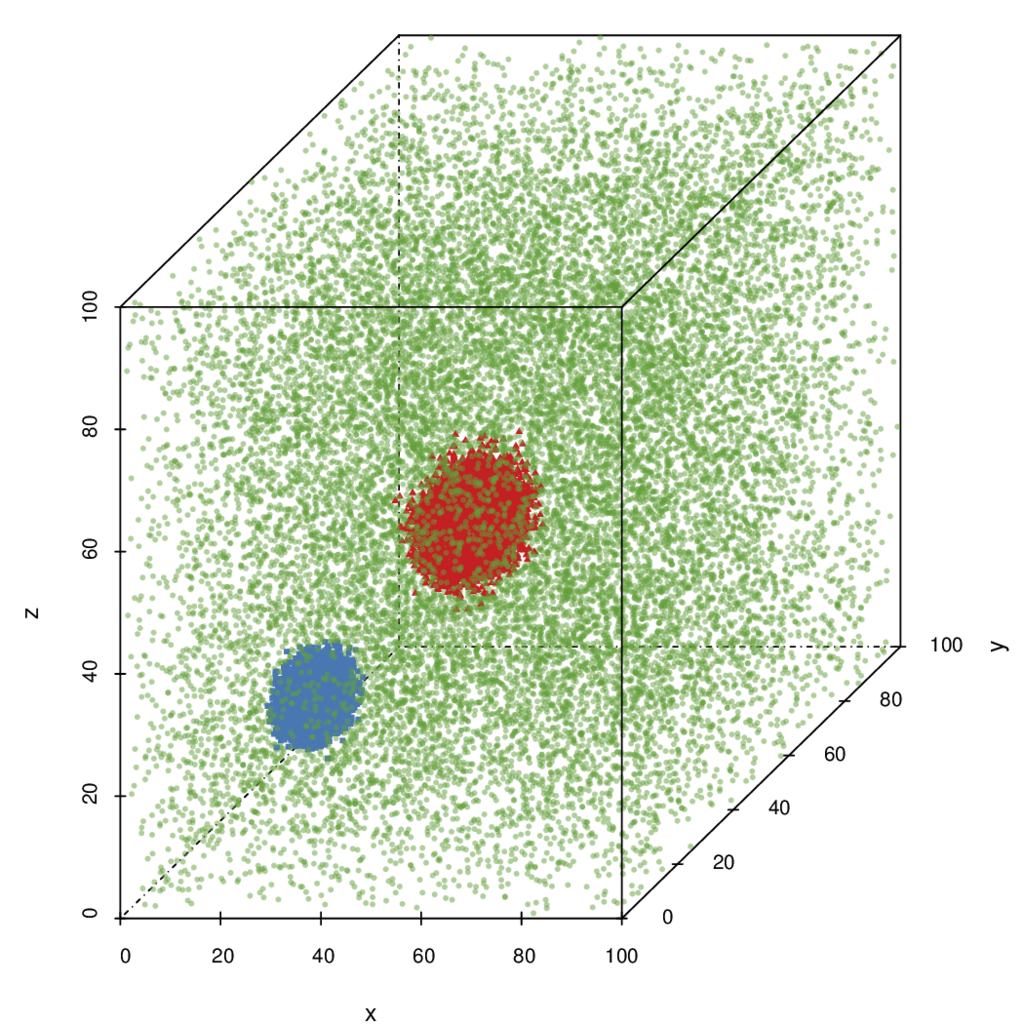
\includegraphics[width=\textwidth]{experiment/img/datasetplot_ferdosi_2_60000}
	\caption{Set \ferdosiTwo}
	\label{fig:experiment:multisphere:ferdosi2}
\end{subfigure}	
% Ferdosi Set 3
\begin{subfigure}{0.23\textwidth}
	\centering
	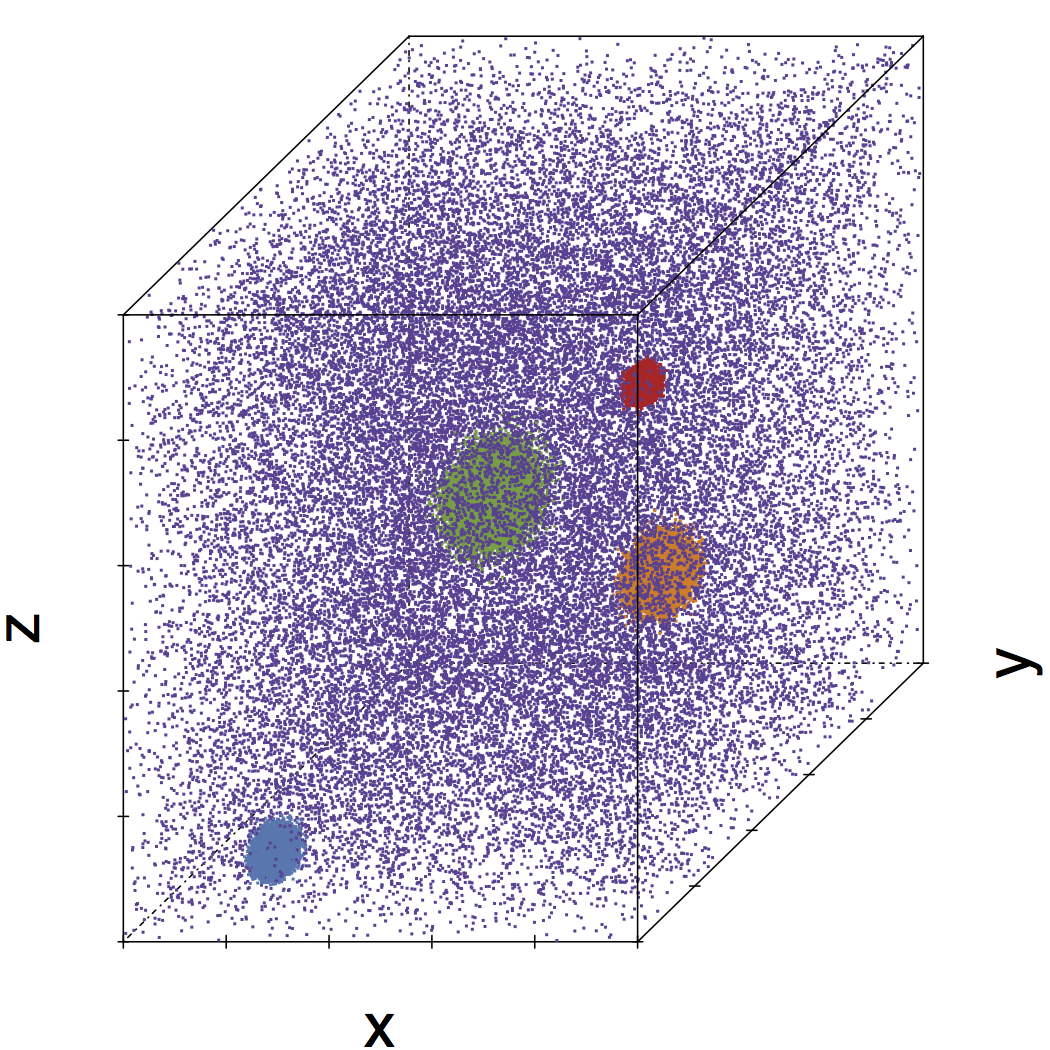
\includegraphics[width=\textwidth]{experiment/img/datasetplot_ferdosi_3_120000}
	\caption{Set \ferdosiThree}
	\label{fig:experiment:multisphere:ferdosi3}
\end{subfigure}	
\subfigvspace
% Baakman 2
\begin{subfigure}{0.23\textwidth}
	\centering
	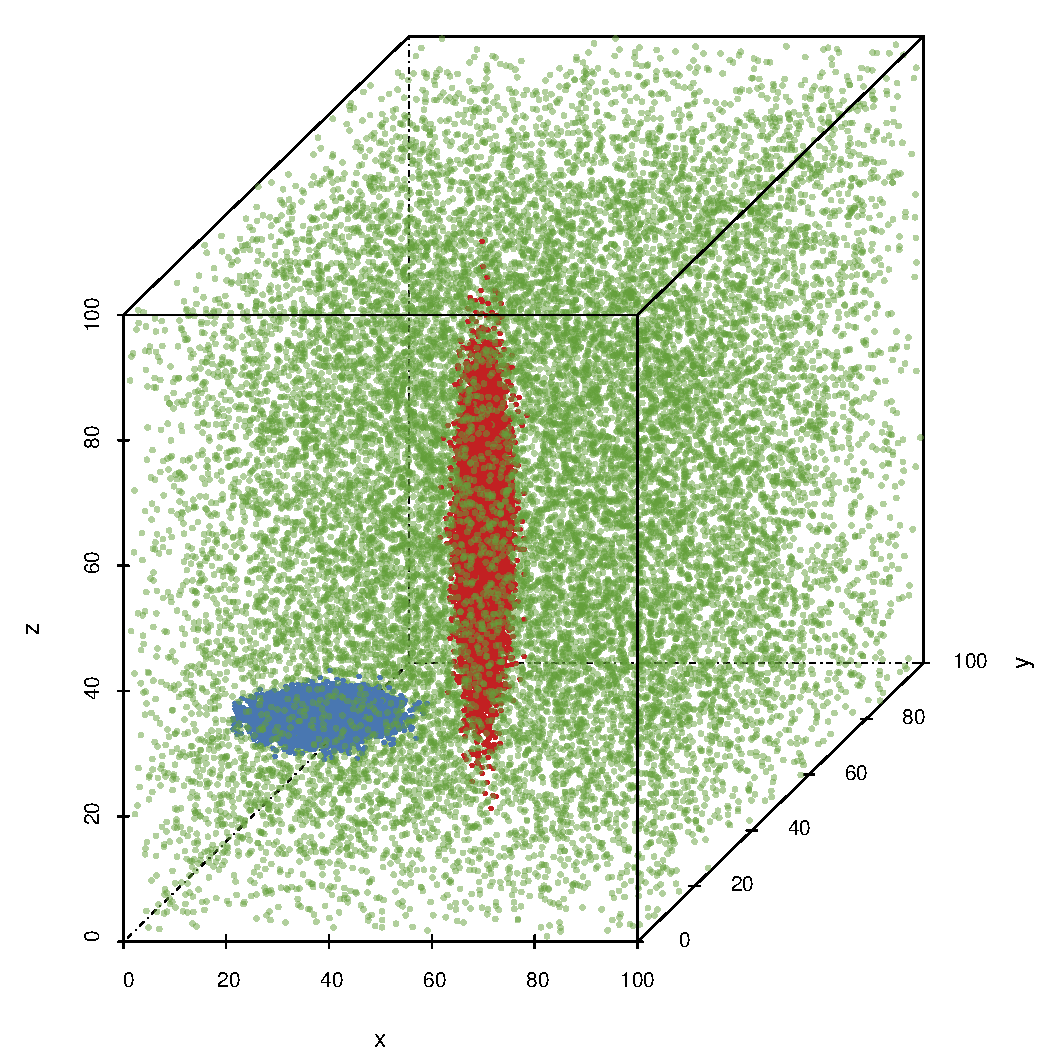
\includegraphics[width=\textwidth]{experiment/img/datasetplot_baakman_2_60000}
	\caption{Set \baakmanTwo}
	\label{fig:experiment:multisphere:baakman2}
\end{subfigure}			
% Baakman 3
\begin{subfigure}{0.23\textwidth}
	\centering
	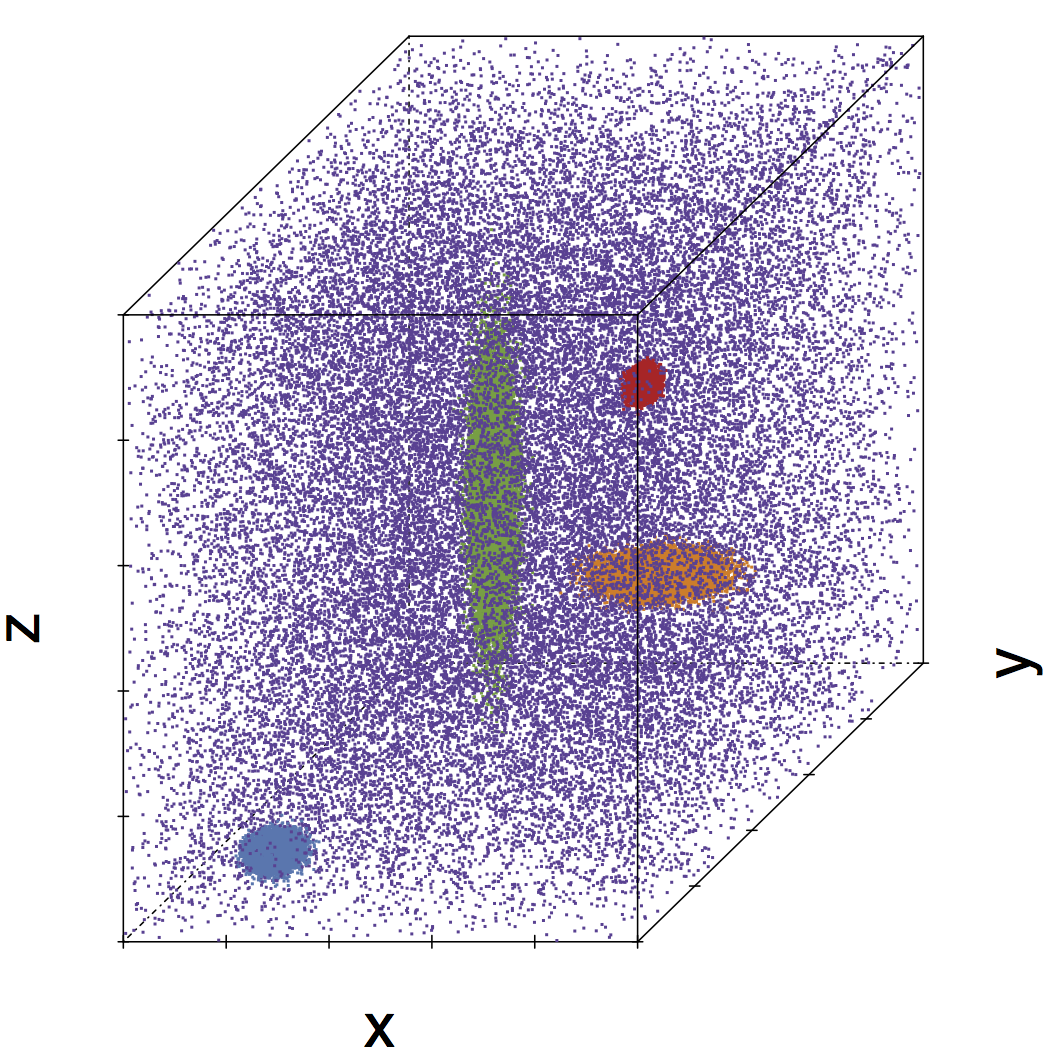
\includegraphics[width=\textwidth]{experiment/img/datasetplot_baakman_3_120000}
	\caption{Set \baakmanThree}
	\label{fig:experiment:multisphere:baakman3}
\end{subfigure}
	\caption{Scatter plot representation of the data sets defined in \cref{tab:experiment:multisphere:sets}, the colors used for the different components correspond to those in \cref{tab:experiment:multisphere:sets}.}
	\label{fig:experiment:multisphere:sets}
\end{figure}

%General
\Cref{tab:experiment:multisphere:sets} defines the data sets that consist of uniform random background and multiple Gaussian distributions. A scatter plot representation of these sets is shown in \cref{fig:experiment:multisphere:sets}.
	% Ferdosi 2
	Data set \ferdosiTwo consists of two Gaussian distributions, that are unlikely to overlap, embedded in an uniform random background. The first Gaussian component is significantly denser than the second.
	% Baakman 2
	The procedure outlined in \cref{s:experiment:singlesphere} for the creation of data set \baakmanOne was used to derive data set \baakmanTwo from \ferdosiTwo.
	% Ferdosi Three
	Data set \ferdosiThree embeds four non-overlapping Gaussians with eigenspheres with notably different radii in the uniform random background.
	%Baakman 3
	The last data set, \baakmanThree, is a variation on \ferdosiThree, created with the method that was used for the definition of data set \baakmanOne from \ferdosiOne.

%Hypothesis
	Due to the spherical nature of the Gaussian components we expect hardly any difference in performance between the estimators on data set \ferdosiTwo and \ferdosiThree. Given the shape of the Gaussian distributions embedded in data set \baakmanTwo and \baakmanThree we hypothesize that \sambe outperforms \mbe on these sets.